%------------------------------------------------------------------------
\begin{frame}
\frametitle{IndexedDB}
\framesubtitle{Client Side Storage}
\begin{columns}[T] % align columns
\begin{column}{.48\textwidth}

\begin{center}
{\Huge IndexedDB}
\end{center}

\end{column}%
\hfill%
\begin{column}{.48\textwidth}
\color{blue}\rule{\linewidth}{4pt}

	\setbeamertemplate{enumerate items}[default]
	\begin{enumerate}
		\item Same Origin Policy (SOP)
		\item Cookies
		\item WebStorage
		\item Application Cache
		\item \textbf{IndexedDB}
	\end{enumerate}
\end{column}%
\end{columns}
\end{frame}
%------------------------------------------------------------------------
\begin{frame}
\frametitle{IndexedDB}
\framesubtitle{Client Side Storage}

Datenbanken im Browser:
\begin{itemize}
	\item WebSQL $\rightarrow$ SQL-Datenbank \\
		Wird nicht als Standard weiterentwickelt.
	\item IndexedDB $ \rightarrow$ NoSQL-Datenbank
\end{itemize}

\end{frame}
%------------------------------------------------------------------------
\begin{frame}
\frametitle{IndexedDB - Fakten}
\framesubtitle{Client Side Storage}

IndexedDB:
\begin{itemize}
	\item Objektspeicher
	\item Erlaubt strukturierte Speicherung von Daten
	\item Implementiert effiziente SCRUD Algorithmen
	\item Keine Speicherung im DOM
	\item SOP
	\item Offiziell keine Größenbeschränkungen	
	\item IndexedDB API asynchron
	\item Event basiertes Benachrichtigungssystem
\end{itemize}

\end{frame}
%------------------------------------------------------------------------
\begin{frame}[fragile]
\frametitle{IndexedDB}
\framesubtitle{Client Side Storage}
	Browser Support
	\begin{center}
		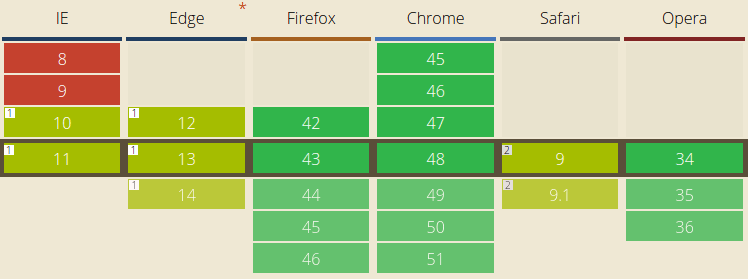
\includegraphics[height=5cm,width=11cm]{img/indexedDB-support.png}
		\\
		
\includegraphics[height=0.5cm,width=5cm]{img/legende.png}
	\end{center}
\end{frame}
\begin{frame}
\frametitle{Quellen}
\framesubtitle{Client Side Storage}

\begin{itemize}
	\item 	\st{JavaScript - Das umfassende Referenzwerk}
	\item Mozilla Developer Network \\
		{\small \url{https://developer.mozilla.org/en-US}/}
	\item Microsoft JavaScript Language Reference \\
		{\small \url{https://msdn.microsoft.com/en-us/library/d1et7k7c(v=vs.94).aspx}}
	\item Canuise.com - Grafiken zur Browserunterstützung \\
		{\small \url{http://caniuse.com/}}
	\item W3C \\
		{\small \url{https://www.w3.org}}
	\item W3CSchools \\
		{\small \url{http://www.w3schools.com/}}	
\end{itemize}
\end{frame}
\begin{frame}
\frametitle{Quellen}
\framesubtitle{Client Side Storage}

Grafiken:
\begin{itemize}
	\item Supercookie: \\  {\small \url{http://www.operationroi.com/wp-content/uploads/2013/11/SuperCookie.jpg}}
	\item Cookie-Monster: \\
	{\small \url{http://www.dearestgeeksofearth.com/wp-content/uploads/2015/02/COOKIE-MONSTER-DEAREST-GEEKS-OF-EARTH.png} }
	\item Javascript -Logo: \\
	{\small \url{https://www.codementor.io/assets/page_img/learn-javascript.png}}
	
\end{itemize}
	Alle Quellen wurden zuletzt am 23.01.15 aufgerufen.

\end{frame}
%------------------------------------------------------------------------